\documentclass[conference]{IEEEtran}
\usepackage[utf8]{inputenc}
\usepackage[spanish]{babel}
\usepackage{amsmath}
\usepackage{amsfonts}
\usepackage{amssymb}
\usepackage{graphicx}
\usepackage[left=2cm,right=2cm,top=2cm,bottom=2cm]{geometry}
\author{\IEEEauthorblockN{Paul Percca, Ivan Sipiran} 
\IEEEauthorblockA{Pontificia Universidad Católica del Perú}
\IEEEauthorblockA{Lima, Perú}
\IEEEauthorblockA{cristian.percca@pucp.edu.pe, isipiran@pucp.edu.pe}
}
\title{Identificación Automática del Comportamiento de Clientes de una Tienda Retail mediante Secuencias de Video utilizando Aprendizaje Profundo}

\begin{document}

\begin{figure}[hbtp]
\centering
\includegraphics[scale=0.8]{Figuras/reporte.png}
\end{figure}

\maketitle

\begin{abstract}
Las tiendas físicas usan múltiples técnicas para analizar el comportamiento del cliente, la mayoría de estas, se centra en la captura de datos en caja, al finalizar el proceso de compra; sin embargo, se pierde información valiosa sobre el cliente, durante su estadía en la tienda. Por lo tanto, identificar las rutas de movimiento que tomaron los clientes dentro de una tienda y conocer el grado de interés de los clientes frente a determinados productos, es importante para los gerentes de tienda, ya que, esos conocimientos pueden ayudar a crear mejores campañas de marketing y publicidad dirigida, así como optimizar el almacenamiento y la operación de la tienda . Este artículo se enfoca en análisis de video en una tienda retail con el fin de identificar las zonas de la tienda con mayor y menor tráfico de clientes así como identificar las zonas con mayor demanda de consumo, es decir productos que son llevados por los clientes, utlizando modelos del estado del arte en deep learning como object detection (YOLOv3) y pose estimation (HRNet).

\end{abstract}

\begin{IEEEkeywords}
Object Detection, YOLOv3, Pose Estimation, HRNet
\end{IEEEkeywords}

\section{Introducción}
Las tiendas retail, realizan una amplia variedad de actividades, muchas de las cuales pueden ser asistidas por análisis de video, como la planificación de diseños de tiendas basadas en estadísticas de ruta de clientes, el recuento de clientes histórico e instantáneo, entradas y salidas de tiendas, colas de pago, entre otras. Cada transacción comercial y paso durante el proceso de compra, genera una gran cantidad de datos \cite{provost2013data}, que pueden generar indicadores para la toma de decisiones.

Entre esas actividades se encuentra la prevención de pérdidas y la medición del nivel de satisfacción de sus clientes. La prevención de pérdidas se clasifica en cuatro grupos primarios: pérdidas internas (trabajadores de la tienda), externas (supuestos clientes, mediante cambio de etiquetas, fraude en la devolución de productos, entre otros), proveedores y administrativas \cite{deyle2015global}.

Por otro lado, muchos clientes se sienten frustrados debido a que no encuentran su producto deseado, ya sea por haber sido colocados en góndolas inadecuadas o en zonas de la tienda que no son muy transitadas, esto generan una mala experiencia al cliente, lo cual se traduce en pérdidas de venta. Si bien se realizan estrategias comerciales y operativas para el posicionamiento de los productos, y estudios de mercado para ello, esta información no se obtiene en tiempo real y muchas veces quedan obsoletas al ser aplicadas.

Hoy en día existen varias soluciones para análisis de datos de e-commerces, sin embargo, no se tiene mucha información de lo que sucede en la tienda física, por lo tanto, esto puede resultar un inconveniente para los administradores de la tienda. Mediante el uso de análisis de video, deep learning y procesamiento de imágenes. se tiene una recopilación más activa de la información \cite{karim2018customer}, información como, cuántos clientes visitan la tienda, cuántos de las personas que entraron a la tienda compraron, cuánto tiempo permaneció una persona en la tienda, cuál fue la trayectoria de un cliente en la tienda, o cuáles son los productos donde la gente se detiene más o menos tiempo a observar, identificar el interés mediante los gestos que muestra un cliente al estar parado frente a un producto específico. Las respuestas a estas preguntas son  información muy importante para la toma decisiones, ya que  se puede tener una visión general y en base a esta información realizar campañas de marketing o reorganizar la ubicación de los productos de ser necesario.

Con la ayuda de Pose Estimation los gerentes de tienda pueden evaluar el nivel de interés del cliente para la mercancía, la postura del cliente, si está de pie, estirando el brazo o agachándose para tomar un producto puede revelar los hábitos del cliente, por ello en el presente proyecto se usarán las grabaciones de cámaras de vigilancia de una tienda retail, sin embargo no es un problema fácil de resolver debido a la oclusión entre las extremidades\cite{liu2018integral}.

El enfoque de este trabajo se centra identificar las zonas de la tienda con mayor y menor tráfico y así como identificar las zonas con mayor demanda de consumo utlizando técnicas del estado del arte en deep learning como son object detection (YOLOv3) tomado de \cite{redmon2018yolov3} y pose estimation (HRNet) tomado de \cite{sun2019deep} esta información va a ser mostrada en heatmaps de manera que, pueda ser de mayor provecho para los gerentes de tienda y así tomar decisiones que ayuden a la recolocación de productos con el fin de aumentar las ventas, así mismo, este análisis se podrá realizar a demanda pudiento conocer el comportamiento de los clientes cuando se requiera.

\section{Antecedentes Teóricos}

\subsection{Redes Neuronales Artificiales (ANN)}
Las redes neuronales artificiales son un paradigma de programación inspirado en la biología que permite a un algoritmo aprender a partir de un conjunto de datos observacionales \cite{nielsen2018neural}. La investigación en este campo ha tenido grandes avances, desde que McCulloch y Pitts propusieron su modelo de neurona \cite{mcculloch1943logical}. Una neurona artificial consta básicamente de un vector entradas $X$ y una matriz de pesos $W$, una función de transferencia $f$  que es el promedio ponderado de las entradas y los pesos: $ f(X) = \sum_{j} X_j W_{i,j}$ , posteriormente se  aplica una función de activación que es una transformación no lineal de la función de transferencia $g$ como una Sigmoidal, Tangente Hiberbólica, ReLU, entre otras, $ g(X) = g(\sum_{j} X_j W_{i,j})$, como se aprecia en la Figura \ref{fig:perceptron} hasta la actualidad donde se cuenta con Deep Learning.
\begin{figure}[hbtp]
\centering
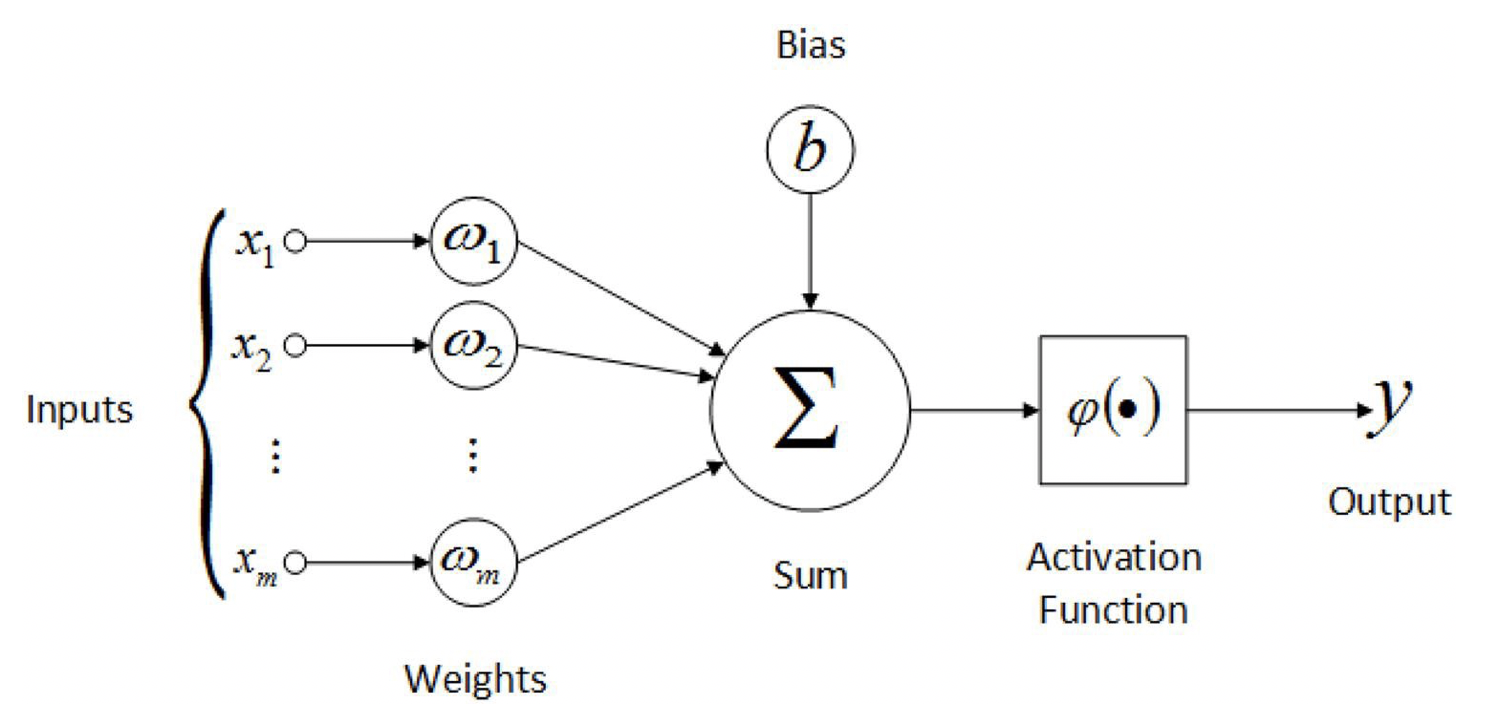
\includegraphics[width=8cm]{Figuras/perceptron.png}
\caption{Modelo de una neurona artificial}
\label{fig:perceptron}
\end{figure}

\subsection{Deep Learning}

Deep Learning permite a modelos computacionales compuestos, por multiples capas de procesamiento, aprender representaciones más complejas con múltiples niveles de abstracción, y todo esto gracias al uso de un algoritmo de backpropagation que permite ir ajustando los pesos hasta las capas anteriores \cite{lecun2015deep}, es decir, Deep Learning es un poderoso conjunto de técnicas para aprender en redes neuronales que proveen las mejores soluciones para muchos problemas en diferentes áreas como reconocimiento de imágenes, reconocimiento de voz y procesamiento de lenguaje natural \cite{nielsen2018neural}. A continuación se muestra un esquema de un modelo de Deep Learning en comparación de una Red Neuronal.

\begin{figure}[hbtp]
\centering
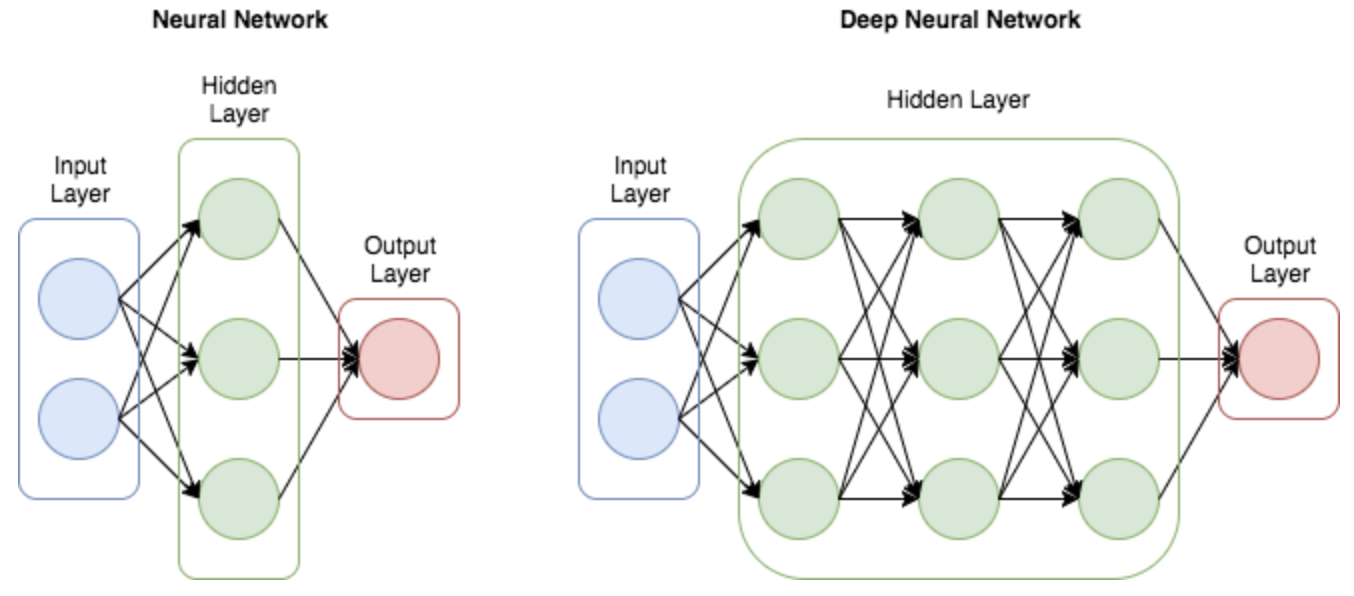
\includegraphics[width=8cm]{Figuras/deeplearning.png}
\caption{Modelo de un Red Neuronal Profunda (Deep Learning)}
\label{fig:deeplearning}
\end{figure}

\subsection{Redes Neuronales Convolucionales (CNN)}
Las Redes Neuronales Convolucionales son un tipo de redes neuronales profundas con aprendizaje supervisado usadas generalmente para procesamiento de imágenes. Las CNN contiene varias capas ocultas especializadas donde las primeras capas pueden detectar lineas, curvas y en sus capas más profundas pueden llegar a reconocer formas complejas como un rostro o la silueta de un animal.
La función lineal usada en este tipo de redes es la convolución, al convolucionar se busca obtener la relación espacial entre la imagen y los diferentes filtros o kernels que se usan, si al operar la ventana o porción de pixeles cercanos de la imagen  y el filtro se obtiene un valor alto, significa que existe una gran correlación entre la sección de imagen y dicho filtro. Por lo general se usa la función de activación ReLU, que permite suprimir la gradiente en el caso sea negativa, además de ello, es computacionalmente eficiente para este tipo de problemas. Las CNN contienen capas de Pooling cuyo objetivo es reducir la dimensionalidad de la data; como el MaxPooling donde se toma el valor máximo de la sección y se elige el valor máximo del filtro que se correlaciona con la imagen, al final del pipeline se usa capas fully connected y se le aplica una función softmax en el caso de un problema de clasificación. A continuación se muestra un ejemplo de un modelo de red Convolucional.

\begin{figure}[hbtp]
\centering
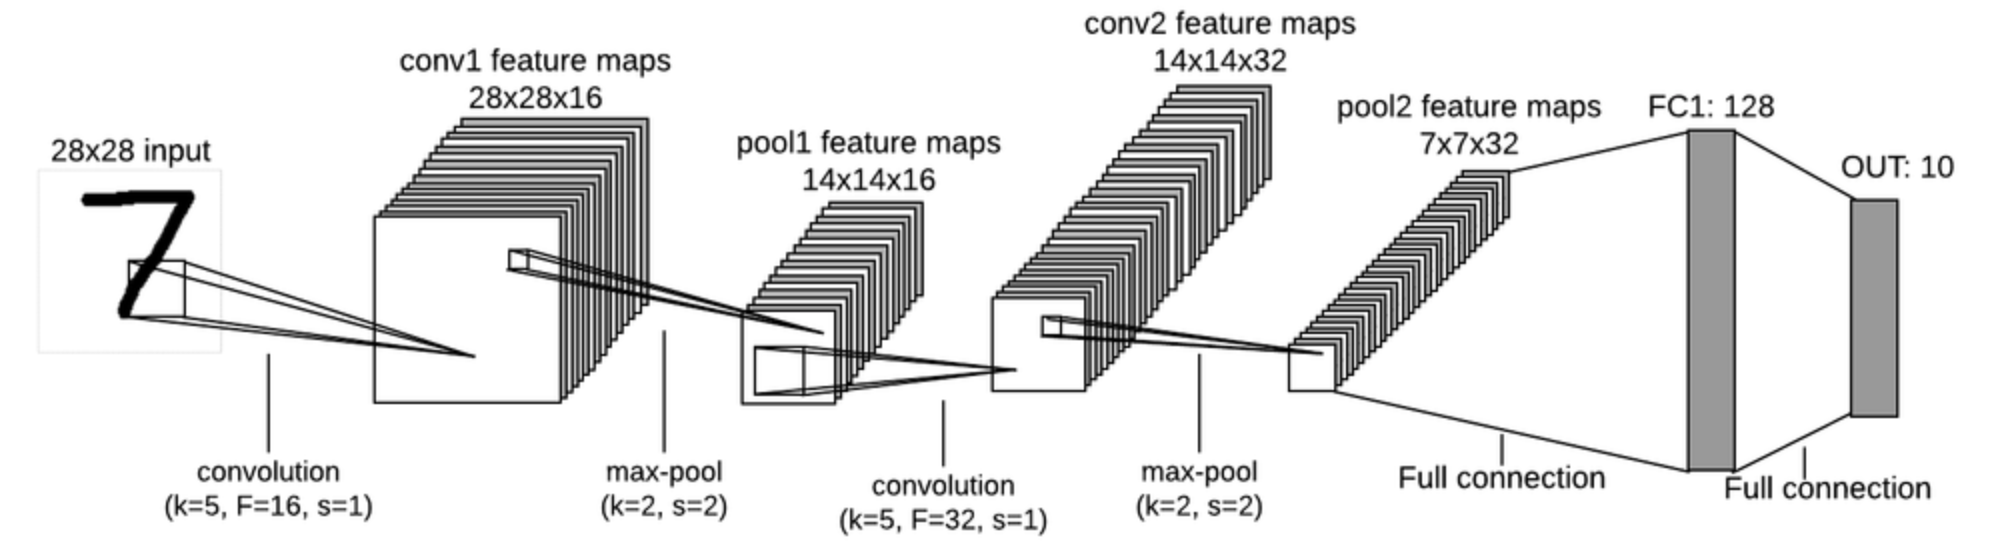
\includegraphics[width=8cm]{Figuras/cnn.png}
\caption{Modelo de una Red Neuronal Convolucional (CNN)}
\label{fig:cnn}
\end{figure}

\subsection{You Only Look Once (YOLO)}

YOLO es un modelo de Red Neuronal Convolucional usada para la detección de objetos que predice simultáneamente múltiples cuadros delimitadores y probabilidades de clase para esos cuadros, si bien YOLO comete más errores de localización, es menos probable que prediga falsos positivos, además de ello es extremadamente rápido, pudiendo correr a 45 fps en su versión base y en una versión fast a 150 fps, y esto debido a que se plantea la detección como un problema de regresión, YOLO ve la imagen completa, codifica mejor la información contextual sobre las clases y su apariencia a diferencia de otros modelos basados en propuestas de ventana deslizante y región. aprende representaciones generalizables de los objetos, al ser entrado con imágenes naturales y luego probado con ilustraciones, supera otros métodos como DPM y R-CNN \cite{redmon2018yolov3}. La arquitectura de este modelo se muestra en la Figura \ref{fig:yolo}

\begin{figure}[hbtp]
\centering
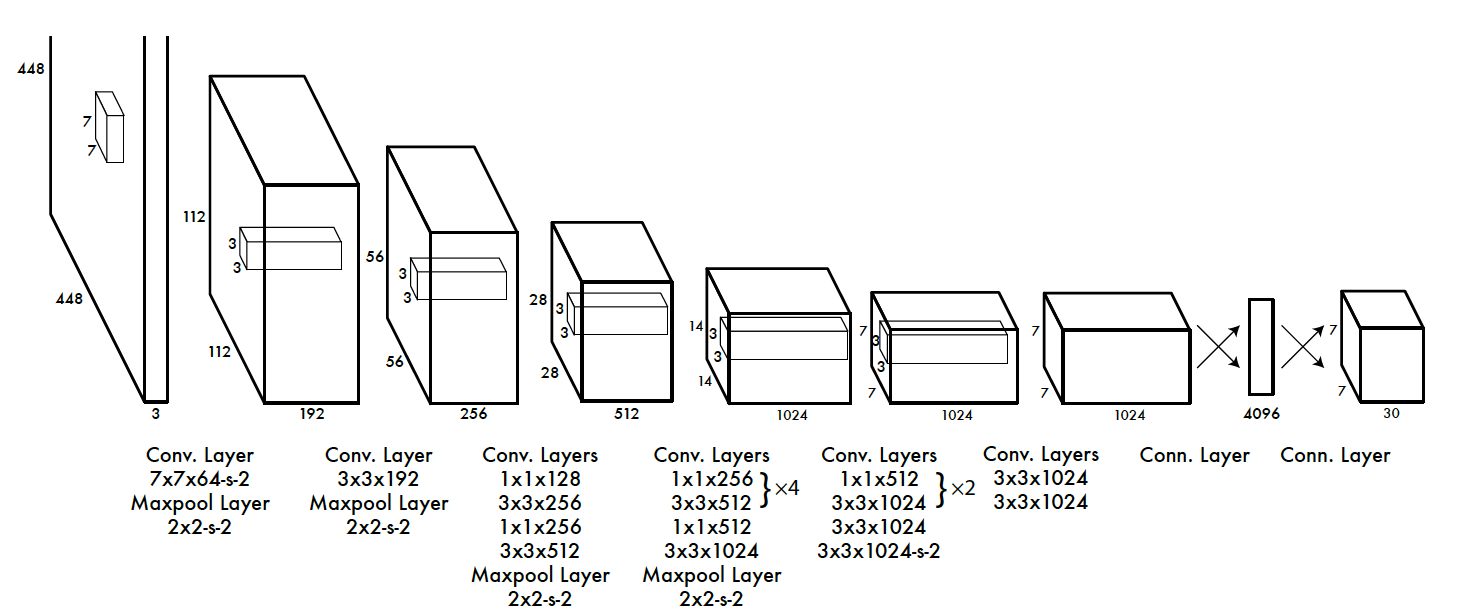
\includegraphics[width=8cm]{Figuras/yolo.png}
\caption{Arquitectura de YOLO}
\label{fig:yolo}
\end{figure}

YOLO divide cada imagen en una cuadrícula de S x S y cada cuadrícula predice B cuadros delimitadores y puntuaciones de confianza, que reflejan la confianza de que el cuadro contiene un objeto y la precisión con la que considera que el cuadro predice, de no haber una imagen en dicha celda, el puntaje es cero. Cada cuadro limitador realiza 5 predicciones x, y, w, h y el puntaje de confianza, donde (x, y) es el centro del cuadro, “w” y “h” son el ancho y el alto que se del objeto que se predice \cite{redmon2018yolov3}.


\subsection{Human Pose Estimation}
Human Pose Estimation consiste en deteminar la posición de las articulaciones humanas o keypoints, como por ejemplo codos, muñecas, rodillas, entre otras. Pose Estimation ha logrado grandes avances gracias a las CNN e incluir un regresor para determinar los heatmaps en la topología de la red neuronal, como se menciona en \cite{bulat2016human}.A continuación se muestra los 15 keypoints usados para estimar la postura humana.

\begin{figure}[hbtp]
\centering
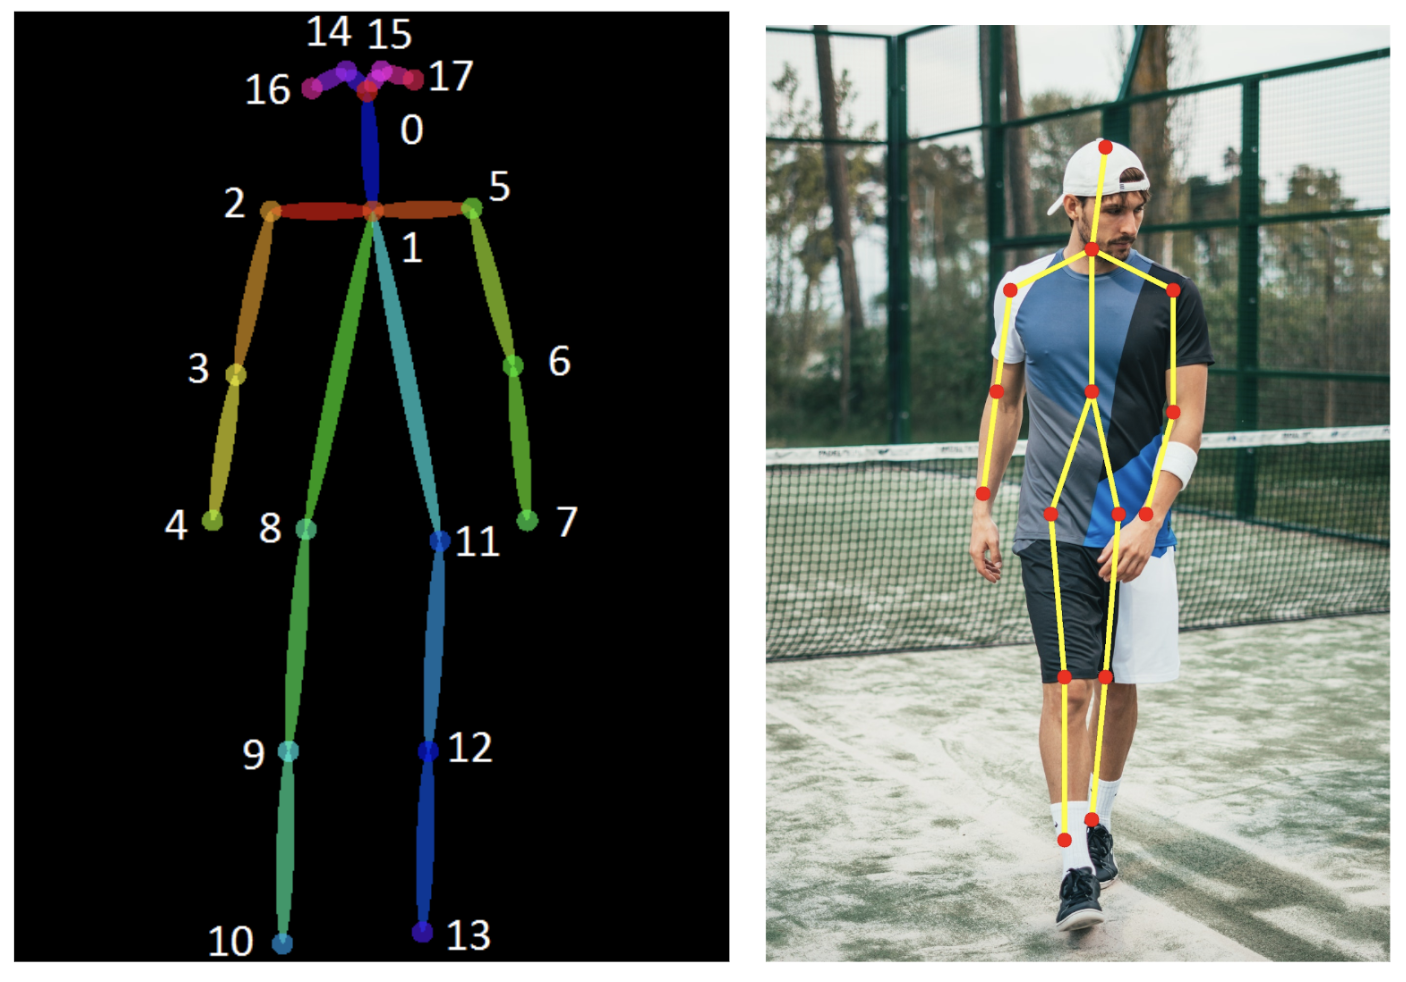
\includegraphics[width=8cm]{Figuras/poseestimation.png}
\caption{Keypoints detectados con Pose Estimation}
\label{fig:poseestimation}
\end{figure}

DeePose \cite{toshev2014deeppose}, fue el primer artículo que aplicó deep learning al problema de Pose Estimation y lo formuló como un problema de regresión basado en CNN para obtener las articulaciones, además de ello se usó una cascada de regresores para mejorar las estimaciones obtenidas, este modelo usa un AlexNet como backbone, con una capa final que calcula los pares de cordenadas $(x, y)$. Las imágenes se recortan alrededor de la articulación pronosticada y se envían a la siguiente etapa, de manera que los regresores posteriores puedan ver las imágenes de mayor resolución obteniendo una mayor precisión. Posteriormente se desarrollaron otros modelos que lograron mejoras en este problema como en \cite{tompson2015efficient} , \cite{wei2016convolutional}, en \cite{carreira2016human} se utiliza un modelo de autocorrección que cambia progresivamente una solución inicial al alimentar las predicciones de error, y este proceso se denomina Retroalimentación de error iterativo (IEF), en \cite{newell2016stacked} donde la red contiene pasos de pooling y capas de upsampling apiladas, lo cual lo asemeja a un reloj , este diseño tiene por objetivo capturar la información a cualquier escala; si bien la muestra local permite identificar características pequeñas, la estimación de la pose requiere un contexto global; y en  \cite{xiao2018simple} donde se usa un modelo Resnet preentrenado con COCO dataset como backbone al cual se le agregan capas deconvolucionales al final del pipeline para estimar los heatmaps, se usa Mean Squared Error como función de pérdida. The HRNet \cite{sun2019deep} , a diferencia de los otros modelos, que iban de representaciones de alta a baja y nuevamente a alta resolución, HRNet conserva la representación en alta resolución durante todo el proces, ya que agrega gradualmente subredes de alta a baja resolución, conectando las subredes multi-resolución en paralelo, obteniendo mejores resultados. 

\section{Trabajos Relacionados}
El análisis de video en el campo de retail, es un tema relevante para los investigadores, incluso grandes  empresas han realizado investigaciones en este rubro:

En \cite{ellis2002performance} se realizó una investigación en procesamiento de video en un contexto retail, basándose en un video grabado en un centro comercial, el objetivo de esta investifación era contar las personas que pasaban y saber cuántas se quedaban frente a un escaparate. De igual manera en \cite{haritaoglu2001detection} se centraron en determinar "grupos de compras" que esperaban en la cola de pago y en \cite{leykin2007detecting} utilizaron algoritmos de enjambre para agrupar clientes "grupos de compras", cabe mencionar que "grupo de compras" es un grupo de persoans que realizarían una compra conjunta, por lo tanto manejar el tráfico del grupo sería un mejor indicativo.

En \cite{senior2007video} IBM planteó un sistema de vigilancia y análisis de video que se centró en la prevención de pérdidas, permitiendo al usuario elegir regiones activas y observar cuántos clientes ingresaron a una región en un período de tiempo, cuántos se detuvieron allí y cuánto tiempo pasaron estos clientes. Se muestran todas las trayectorias de los clientes y permiten al usuario "profundizar" en el video original para observar el comportamiento de los clientes seleccionados. Esta solución consistía en realizar el seguimiento de objetos genéricos y el seguimiento de caras, dicha información de apariencia, trayectoria y fotograma clave del objeto se enviaba a la base de datos, para realizar la clasificación de objetos usaron AdaBoost. Para esta investigación se usaron 6 cámaras, servidores duales Pentium de 3.6GHz para el análisis de video, administración de video y MILS. El algoritmo de seguimiento de ColourField se ejecutaba a 30 fps. La sustracción de fondo toma entre 5,5 y 8,5 ms por fotograma y el seguimiento tomaba entre 2 y 4 ms cuando había un primer plano que se debía seguir.

En la detección de personas también se han realizado investigaciones como:
En \cite{gajjar2017human} donde se realiza una investación en la detección y seguimiento de humanos para videovigilancia con los datos de la Universidad Estatal de Ohio y se incorpora histogramas de gradientes orientados (HOG), la teoría de la prominencia visual y el modelo de predicción de prominencia Deep Multi-Level Network, se usó las funciones HGO para obtener una máquina de vectores de soporte (SVM) para detectar humanos en cualquier frame, para el seguimiento de personas se usó del algoritmo k - means que permitió encontrar los patrones de movimiento en los frames, lo cual es relevante para la reidentificación de la persona. además de ello se usó el algoritmo k - means para comparar y agrupar las características HOG de cuadros consecutivos para identificar el conjunto de puntos en la imagen que se asemejan a una persona en particular que se mueve en el video.

En \cite{liu2018integral} se propone un Integral Pose Network (IntePoseNet) que incorpora la orientación del cuerpo y la máscara de visibilidad, la orientación del cuerpo proporciona la información global de la configuración de pose, además se fusiona con las articulares locales mediante un conjunto de capas novedosas de Orientational Message Passing (OMP) en Deep Neural Network; la máscara de visibilidad modela el estado de oclusión de cada articulación, la orientación del cuerpo es la razón principal de la auto-oclusión, en el dominio temporal, esta red incluye la información del flujo óptico y la estructura BRNN. Por lo tanto, la orientación global del cuerpo, las conexiones conjuntas locales, la información del movimiento humano, el objeto oclusivo y la consistencia temporal se consideran integralmente en la estructura de la red.

\section{Diseño del Experimento}
A continuación se explicará de forma detallada el diseño de la solución presentada en este trabajo de investigación:

Se han usado 5 secuencias de video  de 720 px por 1280 px de cámaras de seguridad para el presente trabajo de investigación tomadas de YouTube, la implementación de los algoritmos se han realizado en Pytorch.

Debido a que se está trabajando con videos, se ha realizado un preprocesamiento, que consiste básicamente en:
\begin{itemize}
\item Remover el audio de los videos.
\item Dividir el video en frames.
\end{itemize}

El desarrollo de la solución se divide en 2 partes que se describen a continuación:
\subsection{Detección de Clientes}
Debido a que la detección de personas es un problema conocido se optó por un modelo de YOLOv3 (Darknet) preentrenado con el dataset COCO 2014.

Luego de realizar el preprocesamiento y de tener los frames separados, con la ayuda del modelo YOLOv3 se ha realizado la detección de personas, y la obtención del bounding box. La posición de la persona $(x, y)$ ha sido determinada como el punto medio del bounding box en el eje $x$ y la posición más baja del bounding box en el eje $y$. Esta coordenada $(x, y)$ ha sido guardadada como la posición del cliente en cada frame. Esta información es calculada a través de la secuencia de videoes como se muestra  graficada en la imagen inferior donde las posiciones del cliente y recorrido se observan como puntos rojos.

\begin{figure}[hbtp]
\centering
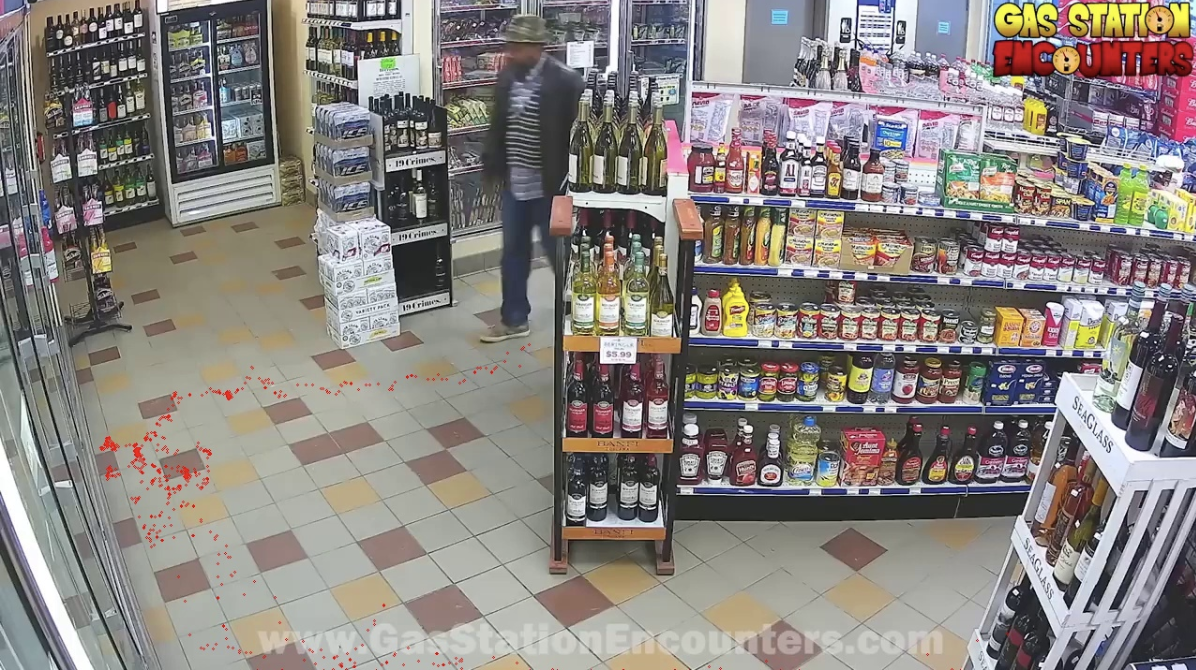
\includegraphics[width=8cm]{Figuras/recorrido.png}
\caption{Recorrido del cliente en la zona de bebidas.}
\label{fig:recorrido}
\end{figure}

Como se aprecia en la figura anterior existe una mayor concentración de puntos en la parte izquierda de la imagen, lo cual indica que la persona ha permanecido una mayor cantidad de tiempo en dicha zona. A continuación se aprecia un heatmap que indica la zona donde el cliente permaneció por un mayor tiempo (zona de bebidas).

\begin{figure}[hbtp]
\centering
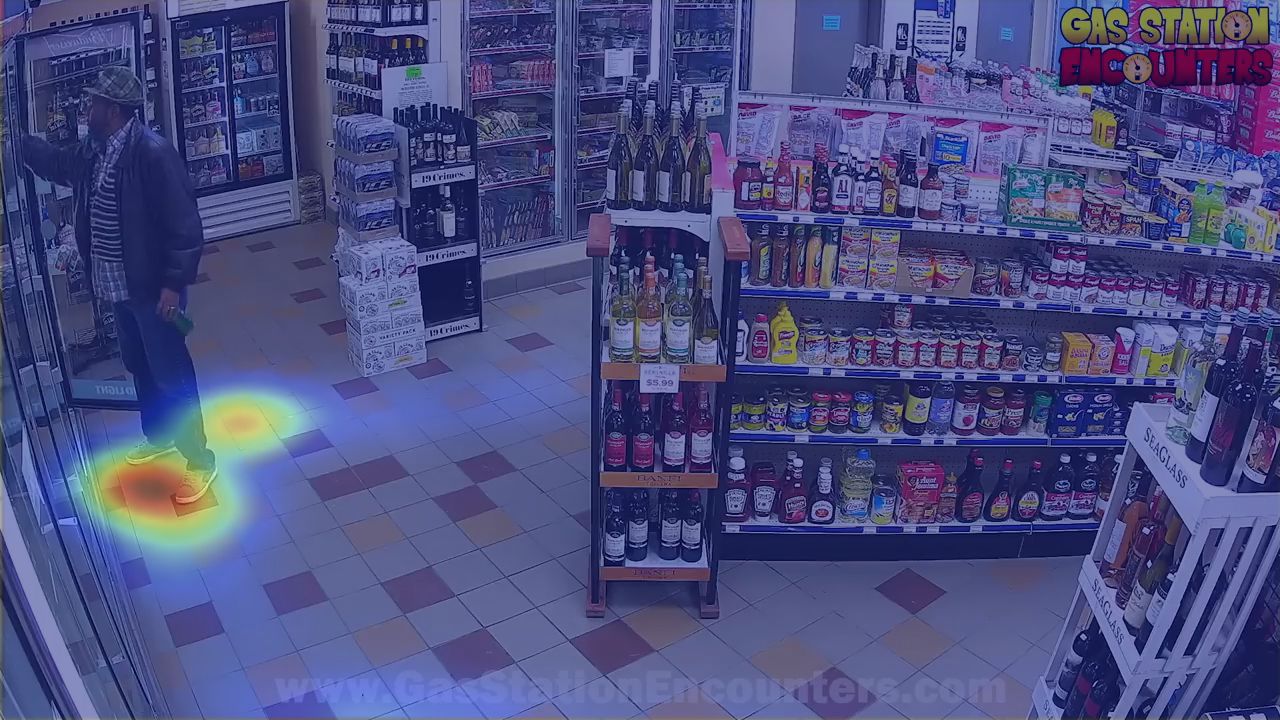
\includegraphics[width=8cm]{Figuras/heatmap.png}
\caption{Heatmap the zonas de consumo dentro de la tienda.}
\label{fig:heatmap}
\end{figure}

\subsection{Human Pose Estimation}
Para la estimación de postura humana del cliente se ha tomado el modelo HRNet \cite{sun2019deep} pre entrenado con COCO 2017, el cual es estado del arte en este campo de Pose Estimation, debido a que mantiene las representaciones de alta resolución durante todo el proceso logrando mejores resultados; con la ayuda de este modelo se obtuvo 15 keypoints (articulaciones) por cada cliente en las imagenes.
Se ha identificado una serie de Posturas Humanas desde diferentes ángulos que indican que el cliente toma un producto de las góndolas de la tienda, el objetivo de esta lista de posturas es comparar las posturas de los clientes obtenidos del video con esta lista de manera que se pueda identificar cuando un cliente toma un producto y guardar la posición $(x, y)$ de este; con esta información se realizará un heatmap indicando las zonas de la tienda donde los clientes se detinen a tomar un producto.

\section{Experimentación y Resultados}

\section{Discusión}

\section{Conclusiones y Trabajos Futuros}

Como trabajos futuros, se plantea aumentar más indicadores con información relevante para la toma de decisiones, así como la implementación de otros modelos de red neuronal, cuyo foco sea la seguridad y la detección de fraudes en las tiendas retail.

\section*{Agradecimientos}

\bibliographystyle{plain}
\bibliography{Bibliografia}

\end{document}